% Construction : la parabole de f(x) = 0,55(x − 2,6)² − 1,4, donc de sommet
% (2,6 ; −1,4) et d'axe de symétrie la droite d'équation x = 2,6.
\begin{tikzpicture}[scale=0.85]
  \draw[->] (-0.4, 0) -- (5.8, 0) node[right] {$x$};
  \draw[->] (0, -2) -- (0, 3.2) node[above] {$y$};
  \draw[thick, domain=0.05:5.15, smooth, variable=\x]
    plot ({\x}, {0.55*(\x - 2.6)*(\x - 2.6) - 1.4});
  \draw[dashed] (2.6, -1.9) -- (2.6, 3);
  \fill (2.6, -1.4) circle (1.6pt);
  \node[below right] at (2.6, -1.4) {$\left(-\tfrac{b}{2a},\ f\!\left(-\tfrac{b}{2a}\right)\right)$};
  \node[above right] at (2.6, 2.6) {axe de symétrie};
\end{tikzpicture}
